\documentclass{article}

\usepackage{geometry}
\geometry{margin=1in}

\usepackage{graphicx}
\graphicspath{}

\title{STAT 778 Homework \#1: a \texttt{C} Implementation of the Kaplan-Meier
Estimator}
\author{Tom Wallace}

\begin{document}

\maketitle

\section{Program Structure}
There are three files. \texttt{misc.c} and its associated header file contain
miscellaneous utility functions (e.g. to create a vector). \texttt{km.c} contains
the \texttt{main} function and is where the more substantive code occurs.

\section{Compiling the Program}
The program uses the \texttt{math.h} standard library and so must be compiled
with the \texttt{-lm} flag. The following is an example of compilation on a
Linux system:

\begin{center}
\texttt{gcc km.c misc.c -lm}
\end{center}

\section{Using the Program}
The program is designed to read in data and output Kaplan-Meier survival
estimates and 95\% confidence intervals. The user must provide input and output
file arguments on the command line. Example:

\begin{center}
\texttt{km -i input\_file -o output\_file}
\end{center}

\section{Verification and Validation}
This program's computed Kaplan-Meier estimates were compared to that obtained
using the \texttt{survival} package in \texttt{R}. Nearly identical results were
obtained, as visualized in Figure 1.

\begin{center}
\begin{figure}[h]
	\caption{Comparison of output}
	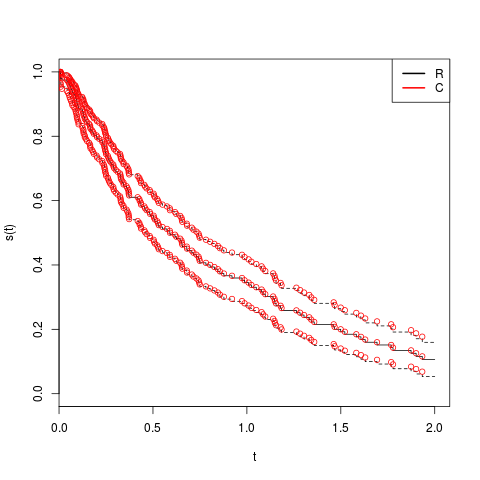
\includegraphics{comparison}
\end{figure}
\end{center}
\end{document}
